This chapter elaborates on the research methodology for the development and evaluation process of an AI-enhanced Web-based MMSE application.

Design Science Research (DSR) is highly suitable for developing and testing such a novel IT artifact in the healthcare sector. DSR is a problem-solving paradigm that seeks to create and evaluate IT artifacts designed to solve identified organizational problems \cite{Hevner2004,Peffers2007}. In the context of AI-powered healthcare solutions, DSR provides a structured framework for addressing complex, multifaceted challenges while ensuring rigorous evaluation and practical relevance \cite{Gregor2013}.

This research adopts a tailored Design Science Research (DSR) methodology, emphasizing four iterative phases, as depicted in Figure \ref{fig:mmse-development-process}:

\begin{figure}[h!]
\begin{center}
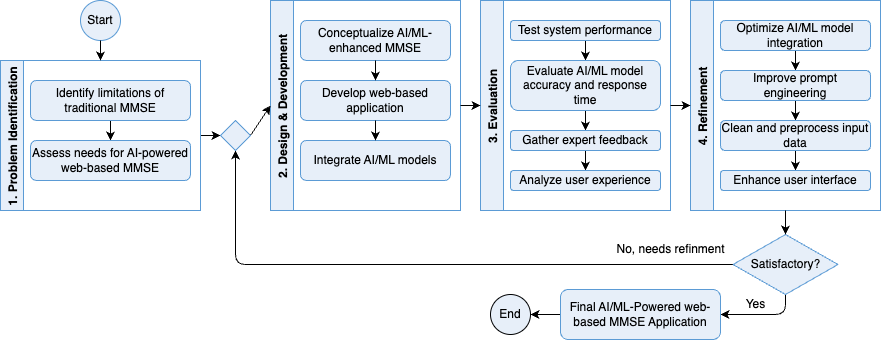
\includegraphics[width=1\textwidth]{theory/figures/flow.drawio.png}
\caption{Iterative development process for the AI/ML-powered web-based MMSE application, illustrating the key stages from problem identification through design, evaluation, and refinement.}
\label{fig:mmse-development-process}
\end{center}
\end{figure}

\begin{enumerate}
    \item \textbf{Problem Identification:} The limitations of traditional MMSE were identified and the needs for an AI-powered web-based MMSE were assessed.
    \item \textbf{Design \& Development:} This phase involved conceptualizing the AI/ML-enhanced MMSE, developing the web-based application, and integrating AI/ML models.
    \item \textbf{Evaluation:} The system's performance was tested, AI/ML model accuracy and response time were evaluated, expert feedback was gathered, and user experience was analyzed.
    \item \textbf{Refinement:} Based on evaluation results, this phase focused on optimizing AI/ML model integration, improving prompt engineering, cleaning and preprocessing input data, and enhancing the user interface.
\end{enumerate}

The process is iterative, with a decision point after the refinement phase to determine if further development is needed. This approach ensures continuous improvement until a satisfactory AI/ML-powered web-based MMSE Application is achieved.

This adaptation of the traditional six-step DSR process was chosen for several key reasons:

\begin{enumerate}
    \item \textbf{Agility and Iteration:} The four-phase cycle allows for quicker iterations, enabling faster response to new AI developments or changing requirements in cognitive assessment tools.
    
    \item \textbf{Focus on Continuous Refinement:} The dedicated 'Refinement' phase and explicit decision point for iteration emphasize the importance of ongoing improvement, which is crucial in AI-powered healthcare applications.
    
    \item \textbf{Integration of AI/ML Specifics:} Each phase explicitly includes AI/ML considerations, ensuring that these aspects are central to the development process.
    
    \item \textbf{Streamlined Process for Time Constraints:} This condensed model allows for a more focused and efficient research process within the time limitations of a master's thesis.
    
    \item \textbf{Alignment with Software Development Practices:} The four-phase cycle mirrors modern software development methodologies like Agile or DevOps, facilitating better integration with real-world development practices.
    
    \item \textbf{Enhanced Flexibility:} This model offers greater flexibility to adapt to the unique challenges of developing an AI-powered cognitive assessment tool.
    
    \item \textbf{Emphasis on Evaluation and User Feedback:} Significant emphasis is placed on both technical performance assessment and user experience analysis, which are crucial for healthcare applications.
\end{enumerate}

This adaptation of DSR maintains the rigorous, problem-solving approach of the original methodology while tailoring it to the specific needs of AI-powered healthcare solution development. It provides a structured yet flexible framework that is well-suited to the complex, iterative nature of developing an AI-enhanced web-based MMSE application.

The following sections will detail each phase of this adapted DSR methodology as applied to the development of the AI-powered web-based MMSE application.

\subsection{Problem Identification}

Designing a Web-based AI-powered MMSE requires understanding the existing challenges to cognitive assessment and the needs of stakeholders. The limitations of traditional MMSE identified earlier provide the context for the proposed solution.

\subsubsection{MMSE Limitations}

Several limitations exist in current MMSE administrations, which reduce its effectiveness and popularity:

\begin{itemize}
    \item \textbf{Time Constraints:} Traditional MMSE administration requires approximately 10–15 minutes per patient, which can be problematic in busy clinical settings \cite{Folstein1975}.
    
    \item \textbf{Scoring Inconsistencies:} Manual scoring introduces the potential for human error and inconsistencies between administrators \cite{Tombaugh1992}.
    
    \item \textbf{Limited Accessibility:} The need for in-person administration restricts access for patients in remote or underserved areas \cite{Bauer2012}.
    
    \item \textbf{Cultural and Educational Bias:} The standard MMSE may not account for cultural differences or varying educational backgrounds, potentially leading to inaccurate assessments \cite{Cullen2007}.
    
    \item \textbf{Lack of Longitudinal Tracking:} Traditional methods often fail to efficiently track cognitive changes over time \cite{Goldberg2015}.
    
    \item \textbf{Limited Sensitivity:} The MMSE may not detect subtle cognitive changes, particularly in early stages of cognitive decline \cite{Mitchell2009}.
\end{itemize}

These limitations underscore the need for an innovative approach to cognitive assessment to address these challenges while maintaining or improving the validity and reliability of the test.

\subsubsection{Needs Assessment}

Based on identified limitations in the literature and analysis of the field, this research compiles a list of key requirements for an AI-powered cognitive assessment tool:
\begin{itemize}
\item \textbf{Efficiency:} Reduce administration time without compromising test validity.
\item \textbf{Standardization:} Ensure consistent test administration and scoring across different settings.
\item \textbf{Accessibility:} Enable remote administration to reach underserved populations.
\item \textbf{Adaptability:} Accommodate cultural and educational differences through dynamic test adjustments.
\item \textbf{Longitudinal Tracking:} Facilitate easy monitoring of cognitive changes over time.
\item \textbf{Data Security:} Implement robust measures to protect patient data and ensure privacy.
\end{itemize}
These requirements guide the development of the AI-powered web-based MMSE. They ensure the tool addresses key needs and overcomes limitations of traditional cognitive assessments identified in the literature.

\subsection{Artifact Design and Development Process}

The AI-powered web-based Mini-Mental State Examination (MMSE) application employs a modern, scalable architecture designed to meet the needs identified in the problem identification phase. This section details the system's design, including its overall architecture, key components, and the assessment process flow.

\subsubsection{Conceptualizing the MMSE and System Design}

The conceptual design of the AI-powered web-based MMSE application involved transforming traditional MMSE tasks into automated versions suitable for digital administration. This process aimed to maintain the integrity of the original assessment \cite{Folstein1975} while leveraging the capabilities of web-based technologies and artificial intelligence \cite{Bauer2012, Zygouris2017}. As cognitive assessment tasks transition from paper-based to web-based administration, it is important to consider the test's psychometric properties and how the digital medium might affect test performance \cite{Geddes2020}. The details of the traditional MMSE tasks are provided in the appendix\footnote{See Appendix \ref{appendix:mmse} for the details of the traditional MMSE tasks.}.

\begin{table}[h]
\centering
\caption{Transformation of MMSE Tasks to Automated Versions}
\begin{tabular}{|p{0.2\textwidth}|p{0.35\textwidth}|p{0.35\textwidth}|}
\hline
\textbf{Task Category} & \textbf{Traditional MMSE} & \textbf{Automated Version} \\
\hline
Orientation & Verbal questions about time and place & Multiple choice questions (QuestionId 2-5, 15), Text input (QuestionId 17-21) \\
\hline
Registration & Verbal repetition of three words & Image recognition and multiple choice (QuestionId 6-8) \\
\hline
Attention and Calculation & Serial subtraction or spelling word backwards & Numeric input for subtraction task (QuestionId 9) \\
\hline
Recall & Recall of three words & Text input (QuestionId 10) \\
\hline
Language & Naming objects & Image recognition with text input (QuestionId 11-12) \\
\hline
Repetition & Repeat a phrase & Voice input and AI transcription (QuestionId 1) \\
\hline
Complex Commands & Three-stage command & Drag and drop interface (QuestionId 16) \\
\hline
Reading & Read and obey a written command & Text input to confirm understanding (QuestionId 13) \\
\hline
Writing & Write a sentence & Text input with AI grammar check (QuestionId 14) \\
\hline
Visuospatial Skills & Copy a design & Drawing interface with AI image analysis (QuestionId 22) \\
\hline
\end{tabular}
\label{tab:mmse-transformation}
\end{table}

\subsubsection{Challenges and Solutions in Automating MMSE Tasks}

Automating the MMSE tasks involved several challenges, requiring careful consideration of the limitations and capabilities of current technology. Below are detailed descriptions of the problems encountered and the solutions implemented for each task category:

\textbf{Orientation:} Traditionally, the tester asks the individual verbal questions related to time and place (e.g., "What is the date today?" or "Where are we right now?"). Points are given based on the accuracy of the responses. In the automated version, multiple choice questions are used to assess these aspects. The system presents questions related to time and place, and the user selects the correct answer from a list of options. This approach ensures accurate scoring and immediate feedback, facilitating the assessment process.

\textbf{Registration:} In the traditional MMSE, the individual is asked to repeat three words (e.g., "apple, penny, table"). The automated version uses image recognition and multiple choice to realize this task. The user is shown images corresponding to the words and must select the correct ones. If the user incorrectly identifies the images, the system provides immediate feedback and logs the response for further evaluation.

\textbf{Attention and Calculation:} Traditionally, tasks like serial subtraction (e.g., subtracting 7 from 100) or spelling words backward are used. In the automated version, numeric input fields are provided for tasks such as subtraction. The system processes the input, checking for correct and incorrect answers, and provides feedback accordingly. Incorrect answers are noted, and hints or step-by-step guidance can be offered to help the user understand the mistake.

\textbf{Recall:} This task involves recalling three previously mentioned words. In the automated version, the user inputs their answers into text fields. The system uses text recognition to evaluate the responses, allowing for common misspellings or variations in phrasing. Correct answers are scored, and incorrect ones prompt the user to try again or move to the next task with feedback.

\textbf{Language:} Naming objects traditionally involves the individual looking at an object and naming it (e.g., "What is this?"). The automated version utilizes image recognition combined with text input. The user views an image and types the name of the object. The system evaluates the input for correctness, taking into account synonyms and common spelling errors.

\textbf{Repetition:} The traditional task requires the individual to repeat a phrase. The automated version uses voice input, and AI transcribes the spoken response. The transcription is then evaluated for accuracy. Incorrect repetitions are flagged, and the user is asked to try again or move on with feedback.

\textbf{Complex Commands:} In the traditional MMSE, this task involves following a series of verbal instructions, such as "Pick up a sheet of paper with your right hand, fold it, and then set it down on the floor" \cite{Folstein1975}. The automated version transforms this into an interactive drag-and-drop interface. Users perform the tasks by dragging items to specified locations as directed. The system tracks each user action, scoring them based on accuracy and providing immediate feedback if any errors occur.

\textbf{Reading:} In this task, the user is required to read and execute a simple written instruction, such as "Close your eyes." The automated system displays the command as on-screen text and asks the user to confirm their understanding. The system then assesses whether the correct action was taken, ensuring that the user has comprehended the instruction.

\textbf{Writing:} Traditionally, the individual writes a sentence. In the automated version, the user inputs the sentence into a text field. The system uses AI to check the grammar and structure of the sentence, providing feedback on any errors and scoring the response accordingly.

\textbf{Visuospatial Skills:} The traditional task involves copying a design. The automated version provides a drawing interface where users draw using a mouse or touchscreen. AI analyzes the drawing for accuracy against a reference design. Feedback is provided based on the correctness and completeness of the drawing.

By addressing these challenges, the MMSE application provides a robust, automated solution for cognitive assessments, leveraging modern web technologies and advanced AI capabilities to ensure accuracy and reliability in its assessments.

\begin{figure}[h!]
\begin{center}
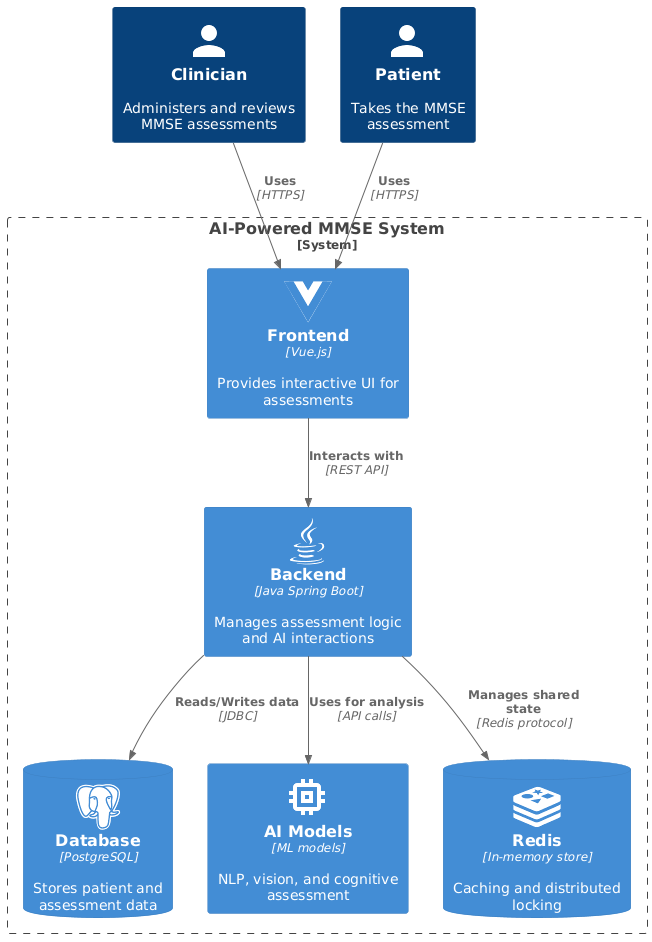
\includegraphics[width=0.80\textwidth]{system-architecture-v3.png}
\caption{Diagram of the AI-Enabled MMSE Application Structure}
\label{fig:system-architecture}
\end{center}
\end{figure}

\subsection{Implementation and Development}

The implementation process of the AI-powered web-based MMSE application followed a structured approach, utilizing modern software engineering practices and technologies. The application was built using a client-server architecture, comprising the following components:
\begin{itemize}
\item Backend: a Java-based Spring Boot application;
\item Frontend: a Vue.js single-page application;
\item Database: PostgreSQL for persistent data storage;
\item External services: AI models (ChatGPT, Ollama with Llama 3.1:70B) for answer evaluation;
\item Caching: Redis for distributed caching and session management;
\item Message queue: RabbitMQ for asynchronous processing.
\end{itemize}

Figure \ref{fig:system-architecture} shows the structure and the AI-powered web-based MMSE application, and also illustrates interactions between clinicians, patients, the frontend and backend components, the database, AI models, and Redis for caching and distributed locking purposes. In the rest of this section, we describe each of these components in more detail.

\paragraph{Backend Design}
The Spring Boot application forms the core of the system, managing business logic, data repositories, and AI service interactions. Key features include:
\begin{itemize}
\item RESTful API with versioning;
\item service layer implementing core business logic;
\item data access layer using Spring Data JPA;
\item integration with external AI services;
\item security implementation with JWT-based authentication;
\item caching and asynchronous processing for improved performance.
\end{itemize}

\paragraph{Frontend Design}
The Vue.js frontend provides a user-friendly interface for both test administrators and test-takers, featuring:
\begin{itemize}
\item responsive design for various devices;
\item state management using Vuex;
\item component-based architecture for maintainability;
\item accessibility features adhering to WCAG guidelines;
\item progressive loading and offline support.
\end{itemize}

\paragraph{Development Environment Setup and Version Control}
GitHub served as the primary version control and collaboration platform, offering robust features that support distributed development and integration with various development tools \cite{github}. The repository structure separated the front- and back-end code, facilitating organized development. JHipster bootstrapped the initial application structure, providing a solid foundation with pre-configured best practices for security, testing, and API development \cite{jhipster}.

\paragraph{Iterative Development Approach and Continuous Integration}
The development process followed an iterative model closely aligned with agile principles. The initial phase involved mapping out all the MMSE questions, which served as the basis for database design and the overall application structure. The development workflow proceeded as follows:
\begin{enumerate}
\item question mapping and requirements analysis;
\item database schema design based on question requirements;
\item implementation of backend services and APIs;
\item frontend component development;
\item integration of AI and machine learning models;
\item continuous testing and refinement.
\end{enumerate}

A GitHub Actions workflow automated the continuous integration (CI) pipeline \cite{github_actions}. This configuration ensured that each commit triggered codebase compilation, execution of unit and integration tests, and performance of code quality checks.

\paragraph{Quality Assurance, Testing, and Dependency Management}
A focused testing strategy maintained high code quality and ensured the reliability of the MMSE application. The testing approach included:
\begin{itemize}
\item \textbf{Unit Testing:} JUnit tested individual components and functions in isolation for the Java back-end, while Jest handled testing for the JavaScript front-end.
\item \textbf{Integration Testing:} Tests for API endpoints and service interactions ensured correct behavior when combining components, particularly for validating the integration of AI models with the application logic.
\item \textbf{Manual Testing:} Regular manual testing sessions verified the user interface, user experience, and general functionality of the application.
\item \textbf{Accessibility Considerations:} The development process incorporated best practices for web accessibility, guided by the Web Content Accessibility Guidelines (WCAG) \cite{wcag}.
\end{itemize}

Dependabot integration into the GitHub repository maintained up-to-date dependencies and addressed potential security vulnerabilities \cite{dependabot}. Dependabot automatically created pull requests to update outdated dependencies, ensuring that the project benefited from the latest library versions and security patches.

\paragraph{Code Quality, Monitoring, and Error Tracking}
Several tools were integrated into the development process to maintain the quality and consistency of the code:
\begin{itemize}
\item ESLint for JavaScript linting;
\item Prettier for code formatting;
\item SonarLint for identifying and fixing code quality issues.
\end{itemize}

These tools were primarily used within the IntelliJ IDEA development environment, providing real-time feedback during coding. ESLint and Prettier configurations were defined in IntelliJ, allowing immediate code style and quality checks as developers wrote the code.

While not implemented in a production environment, the development process considered future monitoring and error tracking:
\begin{itemize}
\item Plans for log aggregation using the ELK stack (Elasticsearch, Logstash, Kibana) aimed at centralized log management and analysis \cite{elk}.
\item Considerations for integration with error tracking services such as Sentry aimed at real-time error monitoring and reporting in production environments \cite{sentry}.
\end{itemize}

\subsubsection{Database and Performance}
The PostgreSQL database schema was designed to efficiently store and retrieve test data, user information, and assessment results. Key entities include:
\begin{itemize}
    \item User management (mmse\_user, mmse\_authority, mmse\_user\_authority);
    \item Test management (test\_entity, user\_answer, patient\_profile, test\_entity\_hash, media\_recording);
    \item AI integration (dolphin\_question, orientation\_to\_place\_answer).
\end{itemize}

This enhanced schema includes relationships and indexing strategies to ensure optimal performance and data integrity. Figure \ref{fig:database-schema} provides a detailed view of the database schema, illustrating the relationships between key entities such as user management, test management, and AI integration components.

\begin{figure}[h!]
\begin{center}
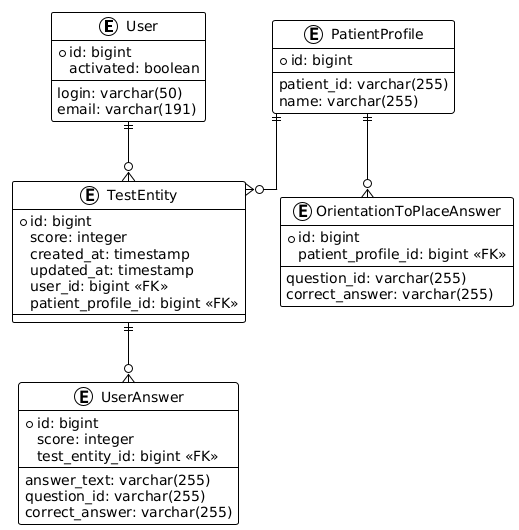
\includegraphics[width=0.65\textwidth]{simplified-database-schema.png}
\caption{Database Schema for the AI-Powered MMSE Application. This schema includes user management, test management, patient profiles, and AI integration.}
\label{fig:database-schema}
\end{center}
\end{figure}

Here is a detailed overview of the primary entities, with the user management section comprising:
\begin{itemize}
    \item \textbf{mmse\_user}: Stores user credentials and profile information.
    \item \textbf{mmse\_authority}: Contains roles and permissions.
    \item \textbf{mmse\_user\_authority}: Links users to their roles.
\end{itemize}

This section related to MMSE testing entities:
\begin{itemize}
    \item \textbf{test\_entity}: Represents individual test instances.
    \item \textbf{user\_answer}: Stores user responses to test questions.
    \item \textbf{patient\_profile}: Contains patient information related to test results.
    \item \textbf{test\_entity\_hash}: Ensures the integrity of the test data with hash values.
    \item \textbf{media\_recording}: Links media files (e.g., audio recordings) to test entities and questions.
\end{itemize}

The \textbf{AI Integration} section includes:
\begin{itemize}
    \item \textbf{dolphin\_question}: Stores questions used in AI-driven assessments.
    \item \textbf{orientation\_to\_place\_answer}: Contains pre-defined answers and options for orientation questions.
\end{itemize}

\paragraph{Performance and Security Enhancements}
While developing the AI-driven web-based MMSE application, performance and security were the highest priorities. This part details the methods employed to enhance database performance, secure data, and sustain solid data flow and integration processes. Additionally, considerations for scalability and upkeep are covered to guarantee the application's efficiency and security over time.

\paragraph{Indexing}
Indexes are created on frequently queried fields such as user\_id, patient\_profile\_id, and timestamps to enhance query performance. Composite indexes are used where appropriate to speed up multi-column searches.

\paragraph{Security}
Data at rest are encrypted using PostgreSQL's native encryption features. Access controls are implemented using roles and permissions to restrict access to sensitive data. Regular backups are scheduled to prevent data loss.

\paragraph{Data Flow}
ETL (Extract, Transform, Load) processes are used to integrate data from various sources into the PostgreSQL database. This ensures a seamless data flow between different components of the system.

\paragraph{Scalability}
The database design considers future scalability with partitioning and sharding strategies. Maintenance is facilitated through regular monitoring and optimization practices.

\paragraph{Security and Privacy Considerations}
The implementation includes robust security measures \cite{owasp2021top10}:
\begin{itemize}
\item JWT-based authentication and role-based access control;
\item strict CORS configuration;
\item comprehensive audit logging;
\item proactive security monitoring.
\end{itemize}

This implementation process ensured the development of a secure, efficient, and user-friendly AI-powered web-based MMSE application, leveraging modern technologies to enhance cognitive assessment practices.

In conclusion, the artifact design and development process for the AI-powered web-based MMSE application leveraged modern software engineering practices to ensure efficient and high-quality development. The combination of iterative development, version control, automated testing, and continuous integration enabled the creation of a reliable and scalable application poised to revolutionize cognitive assessment practices.

\subsubsection{Assessment Process and AI Integration}

The use of the application follows a structured process for administering the MMSE, as illustrated in Figure \ref{fig:assessment-flow}. This process consists of the following steps:

\begin{figure}[h!]
\begin{center}
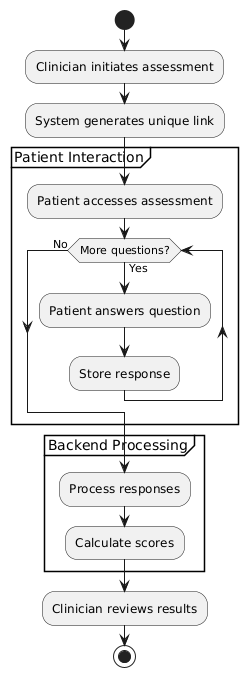
\includegraphics[width=0.34\textwidth]{simplified-flow.png}
\caption{A detailed view of the interactions and data flow during the assessment process.}
\label{fig:assessment-flow}
\end{center}
\end{figure}

\begin{enumerate}
    \item \textbf{Test initiation by the healthcare professional}: The clinician initiates the assessment by generating a unique link for the patient.
    \item \textbf{Patient information collection}: The patient accesses the assessment through the provided link, and the system loads or resumes the current state.
    \item \textbf{Administration of the MMSE through sequential question presentation}: The patient answers various types of questions, including Multiple Choice, Text, Voice, and Drawing. These interactions are captured in the "Patient Interaction" partition of the diagram.
    \item \textbf{Answer collection through various input methods}: Once the patient answers a question, the response is temporarily stored on the frontend. Upon submission of the response by the patient, the system initiates the transition to backend processing. This is a critical juncture in the workflow as indicated by the direct link from "Response Submitted" to the decision node (diamond).
    \item \textbf{AI-powered analysis of patient responses}: At the decision node, the system evaluates whether the submitted response requires AI processing. This decision is based on the type of response and the nature of the question answered by the patient.
    \begin{itemize}
        \item \textit{If AI processing is required}: The system routes the response to the appropriate AI model. For instance:
        \begin{itemize}
            \item \textbf{Llama 3.1:70B} for complex language comprehension.
            \item \textbf{ChatGPT 4o} for processing drawings.
            \item \textbf{Specialized models} for speech-to-text, synonym detection, and semantic understanding.
        \end{itemize}
        \item \textit{If AI processing is not required}: The response undergoes standard processing, bypassing the AI models.
    \end{itemize}
    After processing, whether through AI or standard methods, the response is stored in the database. This ensures that all responses are securely saved for future analysis and score calculation.
    \item \textbf{Generation of clinical insights and result presentation}: Scores are calculated periodically, incorporating concurrency control to manage simultaneous access and updates. This step is crucial for maintaining the integrity and accuracy of the assessment scores. The calculated scores are updated in the database, ensuring that the most recent assessment results are available for review. Finally, the clinician reviews the results of the MMSE, providing a comprehensive overview of the patient’s cognitive state.
\end{enumerate}

This workflow integrates the roles of healthcare professionals, patients, and the AI-enhanced MMSE Tool, ensuring a comprehensive and efficient assessment process.

\subsection{Evaluation Approach}
Assessing the AI-driven web-based MMSE system is essential to verify its efficiency, precision, and user-friendliness compared to conventional techniques. This framework presents a targeted method to evaluate system performance and user interaction through expert assessment \cite{Greenhalgh2017}.

\subsubsection{Performance Indicators}
Experts assess the performance of the AI-powered web-based MMSE application. Key performance indicators (KPIs) include:
\begin{itemize}
\item \textbf{Test Completion Rate:} Percentage of assessments completed without technical issues, as observed by experts.
\item \textbf{Assessment Duration:} Average time taken to complete the MMSE, recorded by experts.
\item \textbf{Score Consistency:} Correlation between AI-generated scores and expert evaluator scores.
\item \textbf{Expert Feedback:} Qualitative feedback from experts on the usability and effectiveness of the web-based system.
\end{itemize}

\subsubsection{Expert Evaluation Process}
A group of 3-5 evaluators with backgrounds in software development and/or user experience design will be recruited to assess the application. The evaluation process will include:
\begin{itemize}
\item \textbf{Comparative Assessment:} Experts will interact with both the AI-powered web-based MMSE and a traditional paper-based MMSE for comparison \cite{Bauer2012}.
\item \textbf{System Usability Scale (SUS):} Evaluators will complete the SUS questionnaire after using the web-based MMSE, providing quantitative feedback on usability and efficiency \cite{Brooke1996}.
\item \textbf{Prototype Testing:} Evaluators will complete a full MMSE assessment using the web-based application, allowing for observations on task completion times and any technical issues encountered \cite{Zygouris2017}.
\end{itemize}

\subsubsection{User Experience Assessment}
To evaluate the user experience of the AI-powered web-based MMSE, we will gather feedback from experts through:
\begin{itemize}
\item \textbf{Semi-structured Interviews:} Brief interviews with the evaluators will capture qualitative insights on the application's strengths, potential areas for improvement, and overall impressions \cite{Wild2021}.
\item \textbf{User Satisfaction Survey:} A survey based on the SUS will assess the overall satisfaction with the web-based system from the perspective of experts \cite{Brooke1996}.
\end{itemize}

\subsubsection{Data Analysis}
Data from this evaluation will be analyzed using basic descriptive statistics for the SUS scores and qualitative analysis of interview responses \cite{Braun2006}. This approach will provide initial insights into the application's usability and potential effectiveness, while also identifying areas for future development and more comprehensive evaluation.

It is important to note that this evaluation is a preliminary assessment and does not constitute a full clinical validation of the tool. A more comprehensive evaluation involving healthcare professionals and a larger, diverse participant group is required for future work \cite{Geddes2020}.